\documentclass{article}
\usepackage[utf8]{inputenc}
\usepackage[margin=0.70in]{geometry}
\usepackage{hyperref}
\usepackage{graphicx}

\title{CS 267: Enabling GPU Support on NumS}
\author{Brian Park, Kunal Agarwal, Parth Baokar}
\date{May 2022}

\begin{document}

\maketitle

\section*{Abstract}
NumS is a library that translates Python and NumPy to optimized distributed systems code. Originally, it was built on top of Ray and was intended for cloud computing environment. We explore how to implement a GPU backend that can be deployable on HPC systems with multi GPU configurations, such as NVIDIA V100 cluster connected with NVLink. We implement a GPU backend that uses CuPy to execute kernels on NVIDIA GPUs and evaluate the performance on multi GPU setup with Ray and NCCL.

\section{Introduction}
Nowadays, there are many parallel primitives that can be used to accelerate numerical workloads. The most popular ones by far for the CPU have been OpenMP, MPI, and UPC++. But often, CPUs do not meet the demand of compute power coming from deep learning models, often requiring petabytes/s of throughput \cite{openai}. Figure \ref{fig:openai} shows that the increase in compute power over the past decade. This is where domain specific hardware is needed, such as GPUs and TPUs to bridge the gap between compute power today's hardware provides and the growing demand from deep learning. But even then, GPUs and TPUs are often limited by high bandwidth memory to store parameters for machine learning. Due to the death of Moore's Law and end of Denard's scaling, distributed systems is often the solution to scale indefinitely. Here, we will analyze and evaluate the performance and design of NumS with single GPU and multi GPU inter-node backends to reach teraflops/s of performance. We will also evaluate the performance gains on machine learning modelling and compare it's performance against CPU backends of NumS

\begin{figure}
  \centerline{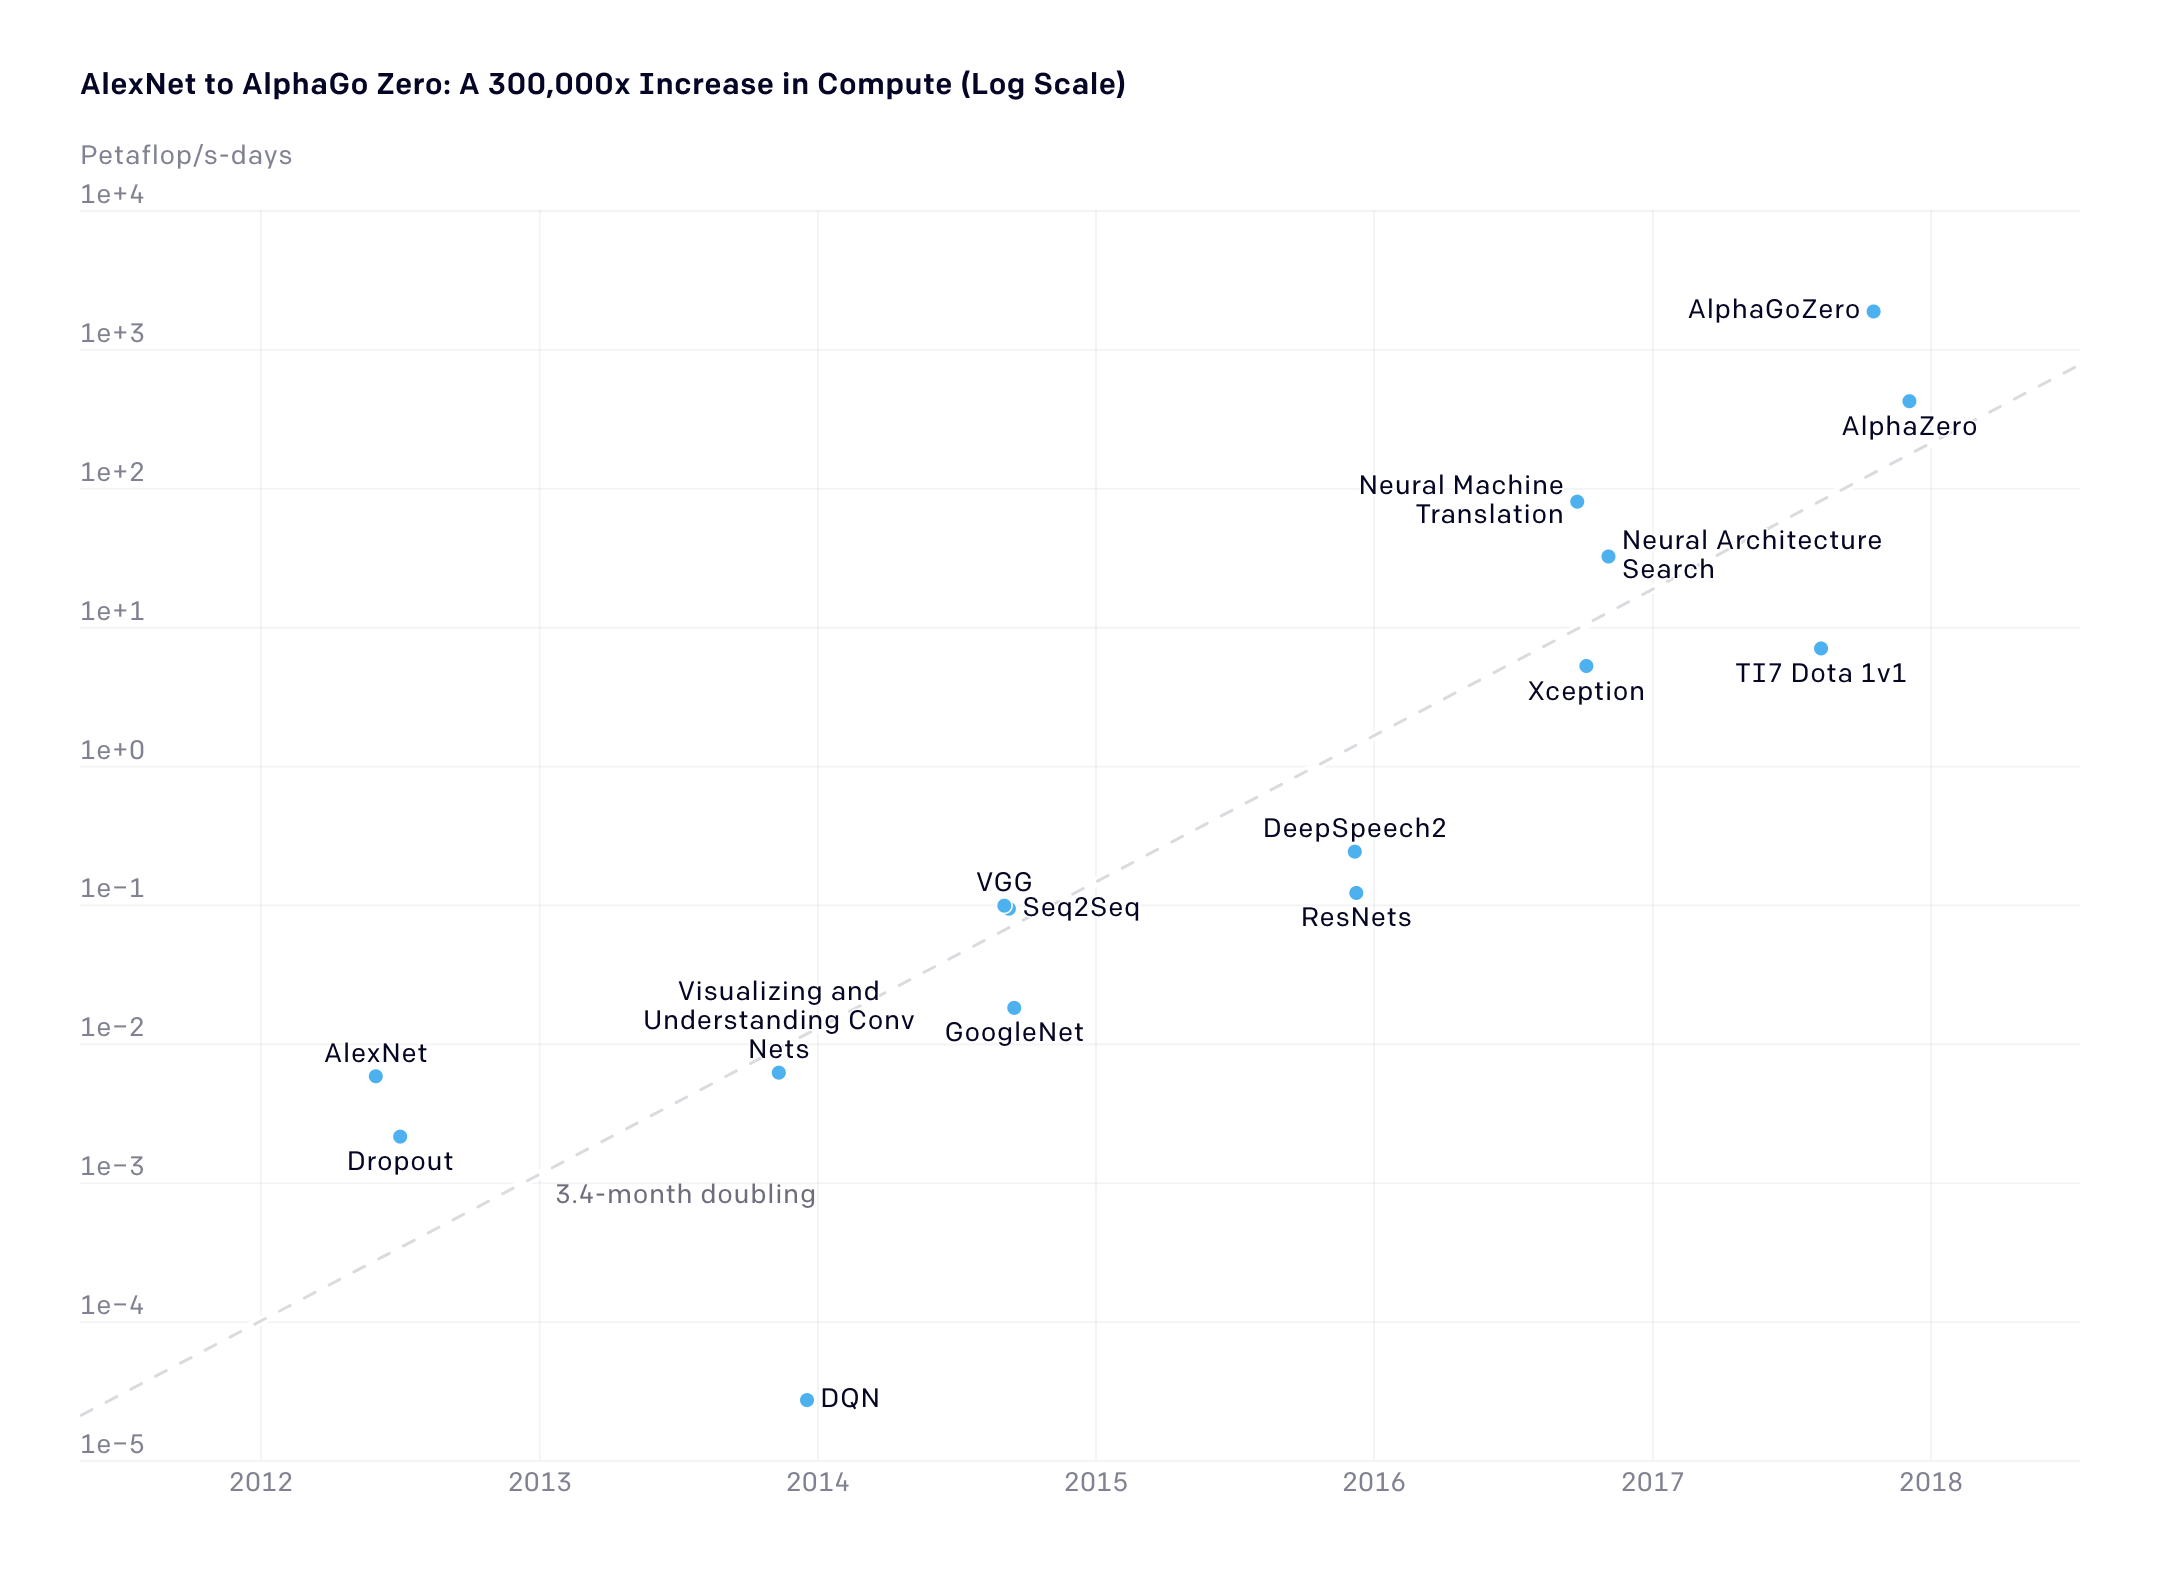
\includegraphics[width=3in]{figures/ai-and-compute-modern-log.png}}
  \caption{Compute Demands of Machine and Deep Learning Models}
  \label{fig:openai}
\end{figure}

\section{Design}
NumS by design already tries to optimize for distributed systems by providing optimal schedulers and communication avoiding algorithms. \cite{nums} We find that these same algorithms can be easily transferable when implementing a multi GPU backend.

The core backend of NumS uses NumPy for numerical computations and it has a kernel interface where computations are executed by partitions in a map-reduce style of programming. NumS has kernels written in NumPy that execute on each data partition in a SPMD style interface. For communication, an application level interface is used to coordinate data movement between devices. Because it was originally written in Ray, the communication APIs are abstracted away from the developer using Ray's object store. The object store is an in-memory distributed object store, using futures and promises to enable task parallelism \cite{ray}. It abstracts away the communication to the developer, making writing distributed programming simple. NumS is able to be aware of array partitioning, placement, and scheduling by utilizing advanced Ray API functionality. In addition to Ray, it also supports a backend for Dask and MPI, so that it could be more easily run on HPC systems. Highlighted in green in Figure \ref{fig:system_arch} is the backends and interfaces implemented in this report.

\begin{figure}
  \centerline{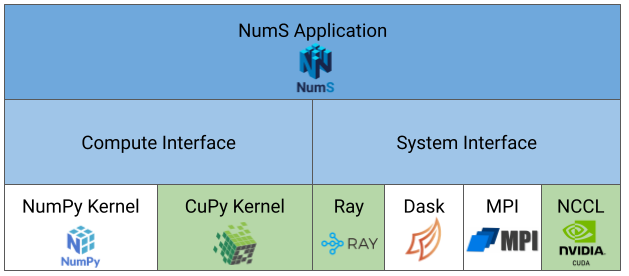
\includegraphics[width=3in]{figures/system_architecture.png}}
  \caption{System Architecture of NumS}
  \label{fig:system_arch}
\end{figure}

CuPy is a NumPy/SciPy-compatible array library for GPU-accelerated computing with Python. It can be often used as drop-in replacement for NumPy, and we use it to enable GPU support on NumS. \cite{cupy} Just like how NumPy can use optimized vendor libraries for BLAS like Intel MKL, CuPy uses NVIDIA's cuBLAS on NVIDIA GPUs while also being aware of NVIDIA hardware features such as NVIDIA Tensor Cores. Thus, CuPy serves as a viable option for NumS compared to other Python array libraries like Dask, Jax, or Numba. This also means that the scope of GPU support on NumS is only limited to NVIDIA GPUs with CUDA support.

Another reason why CuPy serves as a viable option is because it also provides low level CUDA API support such as Python wrappers over the NCCL library. This allows us to write distributed code for NVIDIA GPUs using NCCL as opposed to other options such as CUDA-aware MPI. Another benefit of using NCCL is that it can be used in a single process, where it wont be a problem with Python's global interpreter lock.

Here, we'll explore how we implement GPU support with one GPU and extend it to two more approaches when implementing multi-GPU support with Ray and NCCL. We chose to explore Ray in order to be faithful with the already existing CPU Ray implementation of NumS.

\subsection{Serial}
We implemented the simple serial model, where NumS only uses 1 GPU. This implementation was very simple to implement as we used CuPy as our kernel interface. Properly implementing this gave us a starting point before we extended it to a multi GPU setup. Some basic synchronization primitives have to be implemented such as synchronizing GPU threads and only transferring from GPU memory to main memory when results are needed to be served to the user.

\subsection{Ray}
For implementing the multi-GPU support, we find that Ray's features to abstract away distributed code to the developer and user can be a drawback. Ray's Object Store was meant to be a way to provide a fault tolerant distributed memory model. \cite{ray} This causes a huge latency when doing computations on the GPUs, as Ray enabled functions with CuPy would forcefully route data transfers from CPU to GPU and back from GPU to CPU. This is because Ray exclusively models the Object Store as main memory, and does not include GPU memory in the model. Because low level control is abstracted away, such as explicitly transferring data between nodes or scheduling operations, implementing a high performance GPU backend becomes more of a challenge to implement. Ray was also meant to accelerate task parallelism. Although NumS is successfully able to use Ray features to enable data parallelism computations, Ray's features for data parallelism with GPU is not well supported yet. Ray also provides a collective communication library that can use NCCL to bypass data transfers to the object store. It seems to be successful in Alpa, where they use stateful Ray actor implementations \cite{alpa}. But the design of NumS was built on top of Ray remote functions which are stateless. Trying to incorporate an actor implementation would require a redesign of the NumS system architecture. 

\subsection{NCCL}
With NCCL communication, there are some disadvantages over Ray that NCCL does not supply, such as not being fault tolerant and being susceptible to a deadlock. If a device goes offline in the middle of communication call, this is where NCCL fails to continue, while a Ray implementation can continue on. But since the focus of this implementation was to make NumS deployable under a HPC environment, NCCL served as a better choice in this use case, as these problems are more susceptible in cloud computing. 

When using NCCL, we also had to use multiple CUDA streams to enable concurrency. Naively running code on multiple GPUs will all sync up to the null thread and serialize the timeline and not enable concurrency. For communication under NCCL, we used simple send and receive calls. For future work, we could try to improve the collective communication calls for certain algorithms to utilize other collective calls such as \verb|BCast| and \verb|AllReduce|.

For scalability, we find that we cannot scale easily to more than 4 GPUs. It's susceptible that it may be due to higher latency and 
Figure \ref{fig:nvlink} shows the NVLink mappings and we see longer traversal of communication if a GPU on the left side wants to communicate with the right side. 

\begin{figure}
  \centerline{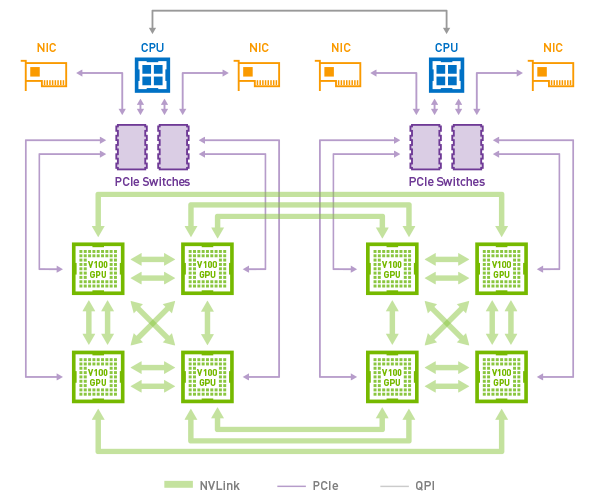
\includegraphics[width=5in]{figures/nvlink.png}}
  \caption{NVLink Mappings in DGX-2 System}
  \label{fig:nvlink}
\end{figure}

\section{Evaluation}
This is one of the first applications where NumS has successfully run on a HPC machine environment. Ray was not intended to run on HPC systems, as mentioned in a guest lecture by Ion Stoica. \cite{ray-lecture}

\subsection{Profiling}
When naively using just the null CUDA stream, we see that concurrency won't be enabled as shown in figure 3

\begin{figure}
  \centerline{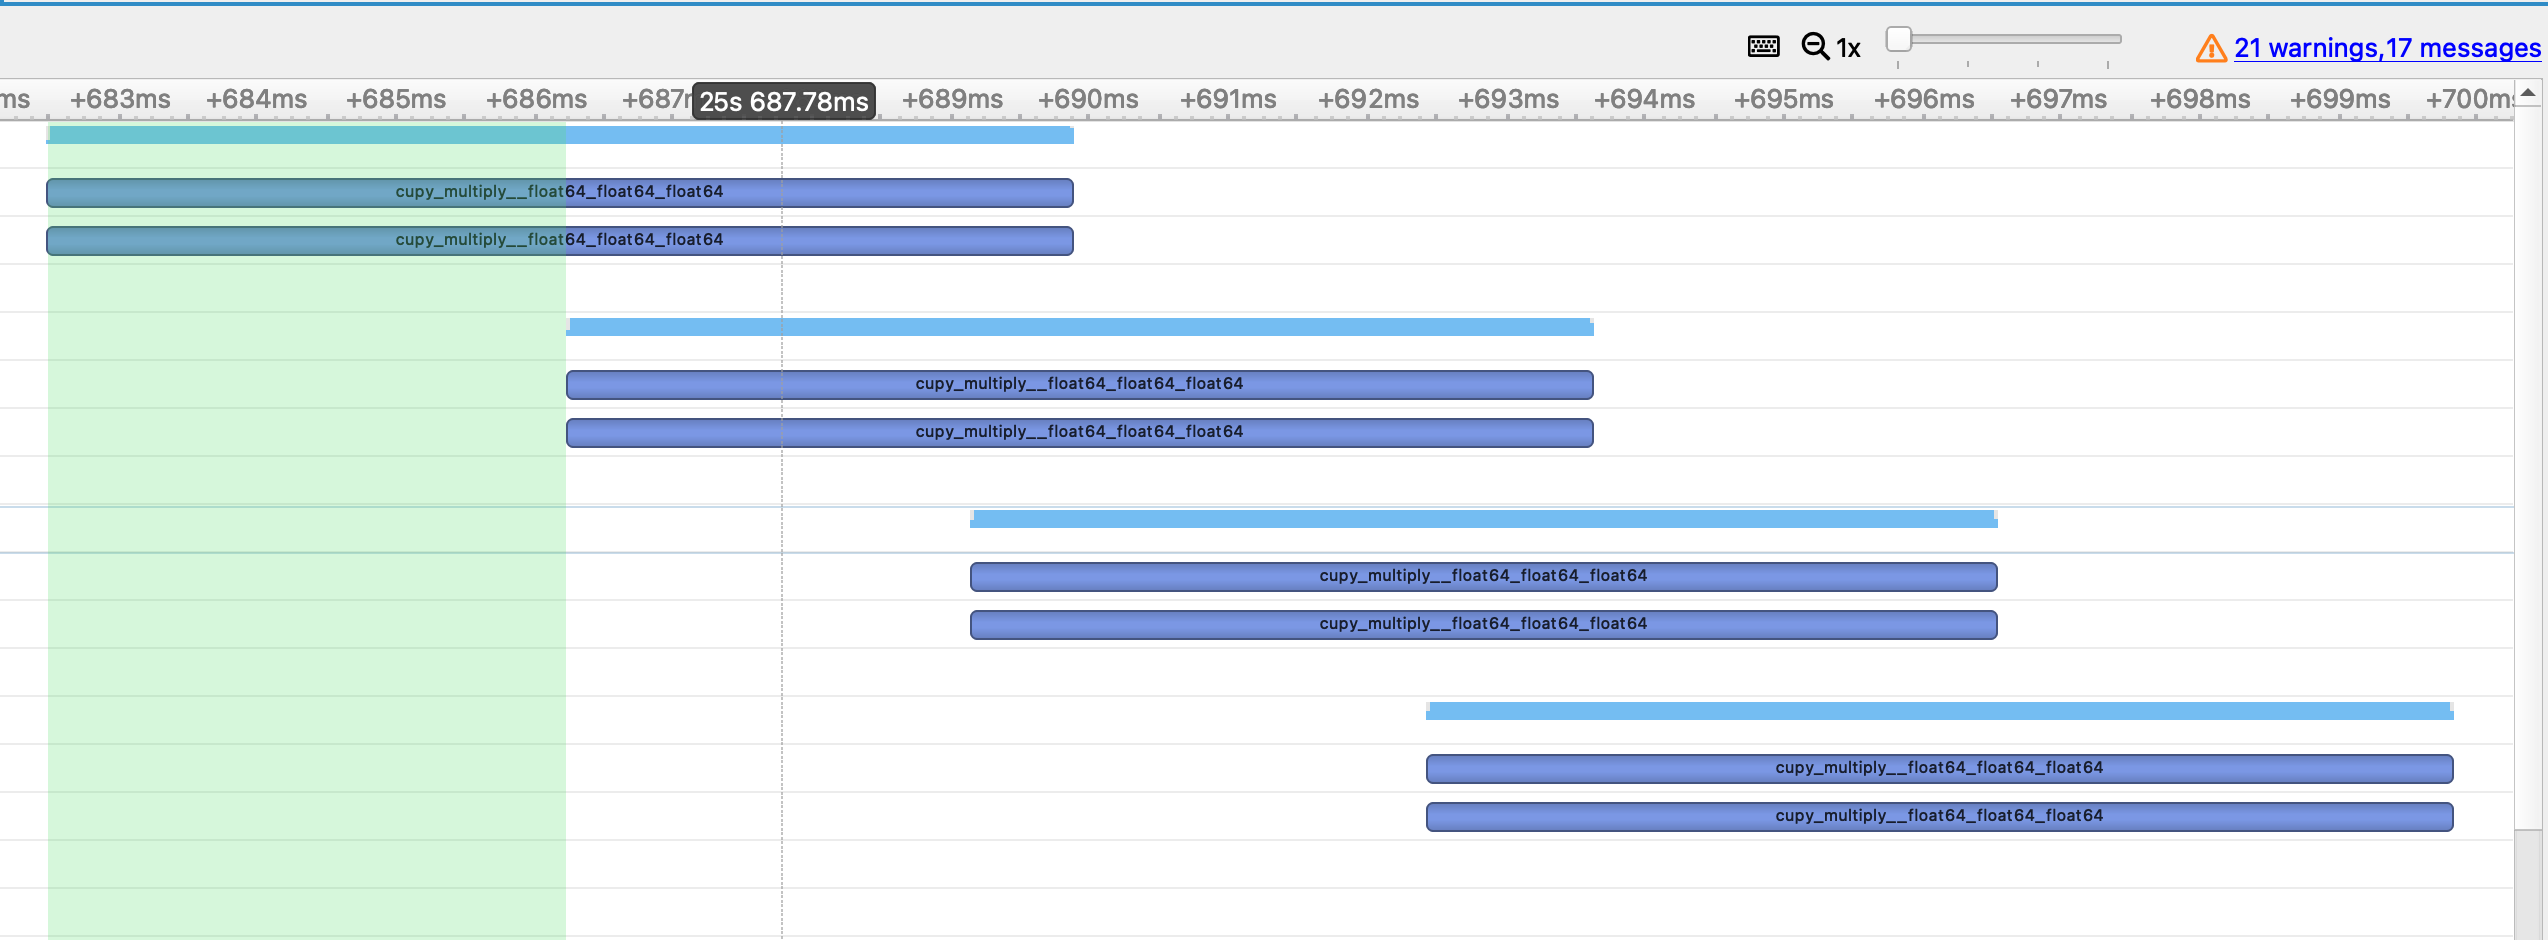
\includegraphics[width=6in]{figures/stream.png}}
  \caption{Streams not being scheduled concurrently}
\end{figure}

\subsection{Benchmarks}
Benchmarking was done on Pittsburgh Supercomputing Center's Bridges-2. They have a \verb|GPU-shared| node that uses up to 8 NVIDIA Tesla V100-32GB SXM2 GPUs and two Intel Xeon Gold 6248 “Cascade Lake” CPUs (20 cores, 2.50–3.90GHz, 27.5MB LLC, 6 memory channels) \cite{psc}. The GPUs are linked with NVLink, which provide 25 Gb/s of bandwidth.


For each benchmark we seeded the random value at every iteration and generated 2 random $n \times n$ matrices to compute $C =  A \times B$. 15 trials per each size is done and the first 5 results are thrown away. This is due to CuPy initializing a CUDA context upon every first CUDA API call. Then the mean of the 10 results are taken and logged.

\subsection{DGEMM}
For a single GPU, William analyzes the Roofline model of V100 architecture theoretically and empirically. The theoretical peak observed for double precision floating point operations in NVIDIA V100 is 7833.6 GFLOP/s while the empirical peak is 7068.9 GFLOP/s \cite{roofline}. We observe by using CuPy's cuBLAS, it will reach near theoretical peak (94.16\%) and almost perfect empirical peak (103.91\%). We suspect that the performance overachieving empirical peak may be due to inaccuracy of timing between Python and CUDA interface that CuPy provides, or the fact that William used \verb|nvprof| and there is profiling overhead collected in the empirical peak. Figure \ref{fig:dgemm} shows the performance of NumS on multiple GPUs. NumS peak performance of each GPU setting maintains 89.2-99.86\% of the empirical peak and 80.84-90.50\% of the theoretical peak. The efficiency decreases as we increase to more GPUs, and this is likely due to communication overhead.

%TODO weak scaling plots
\begin{figure}
  \centerline{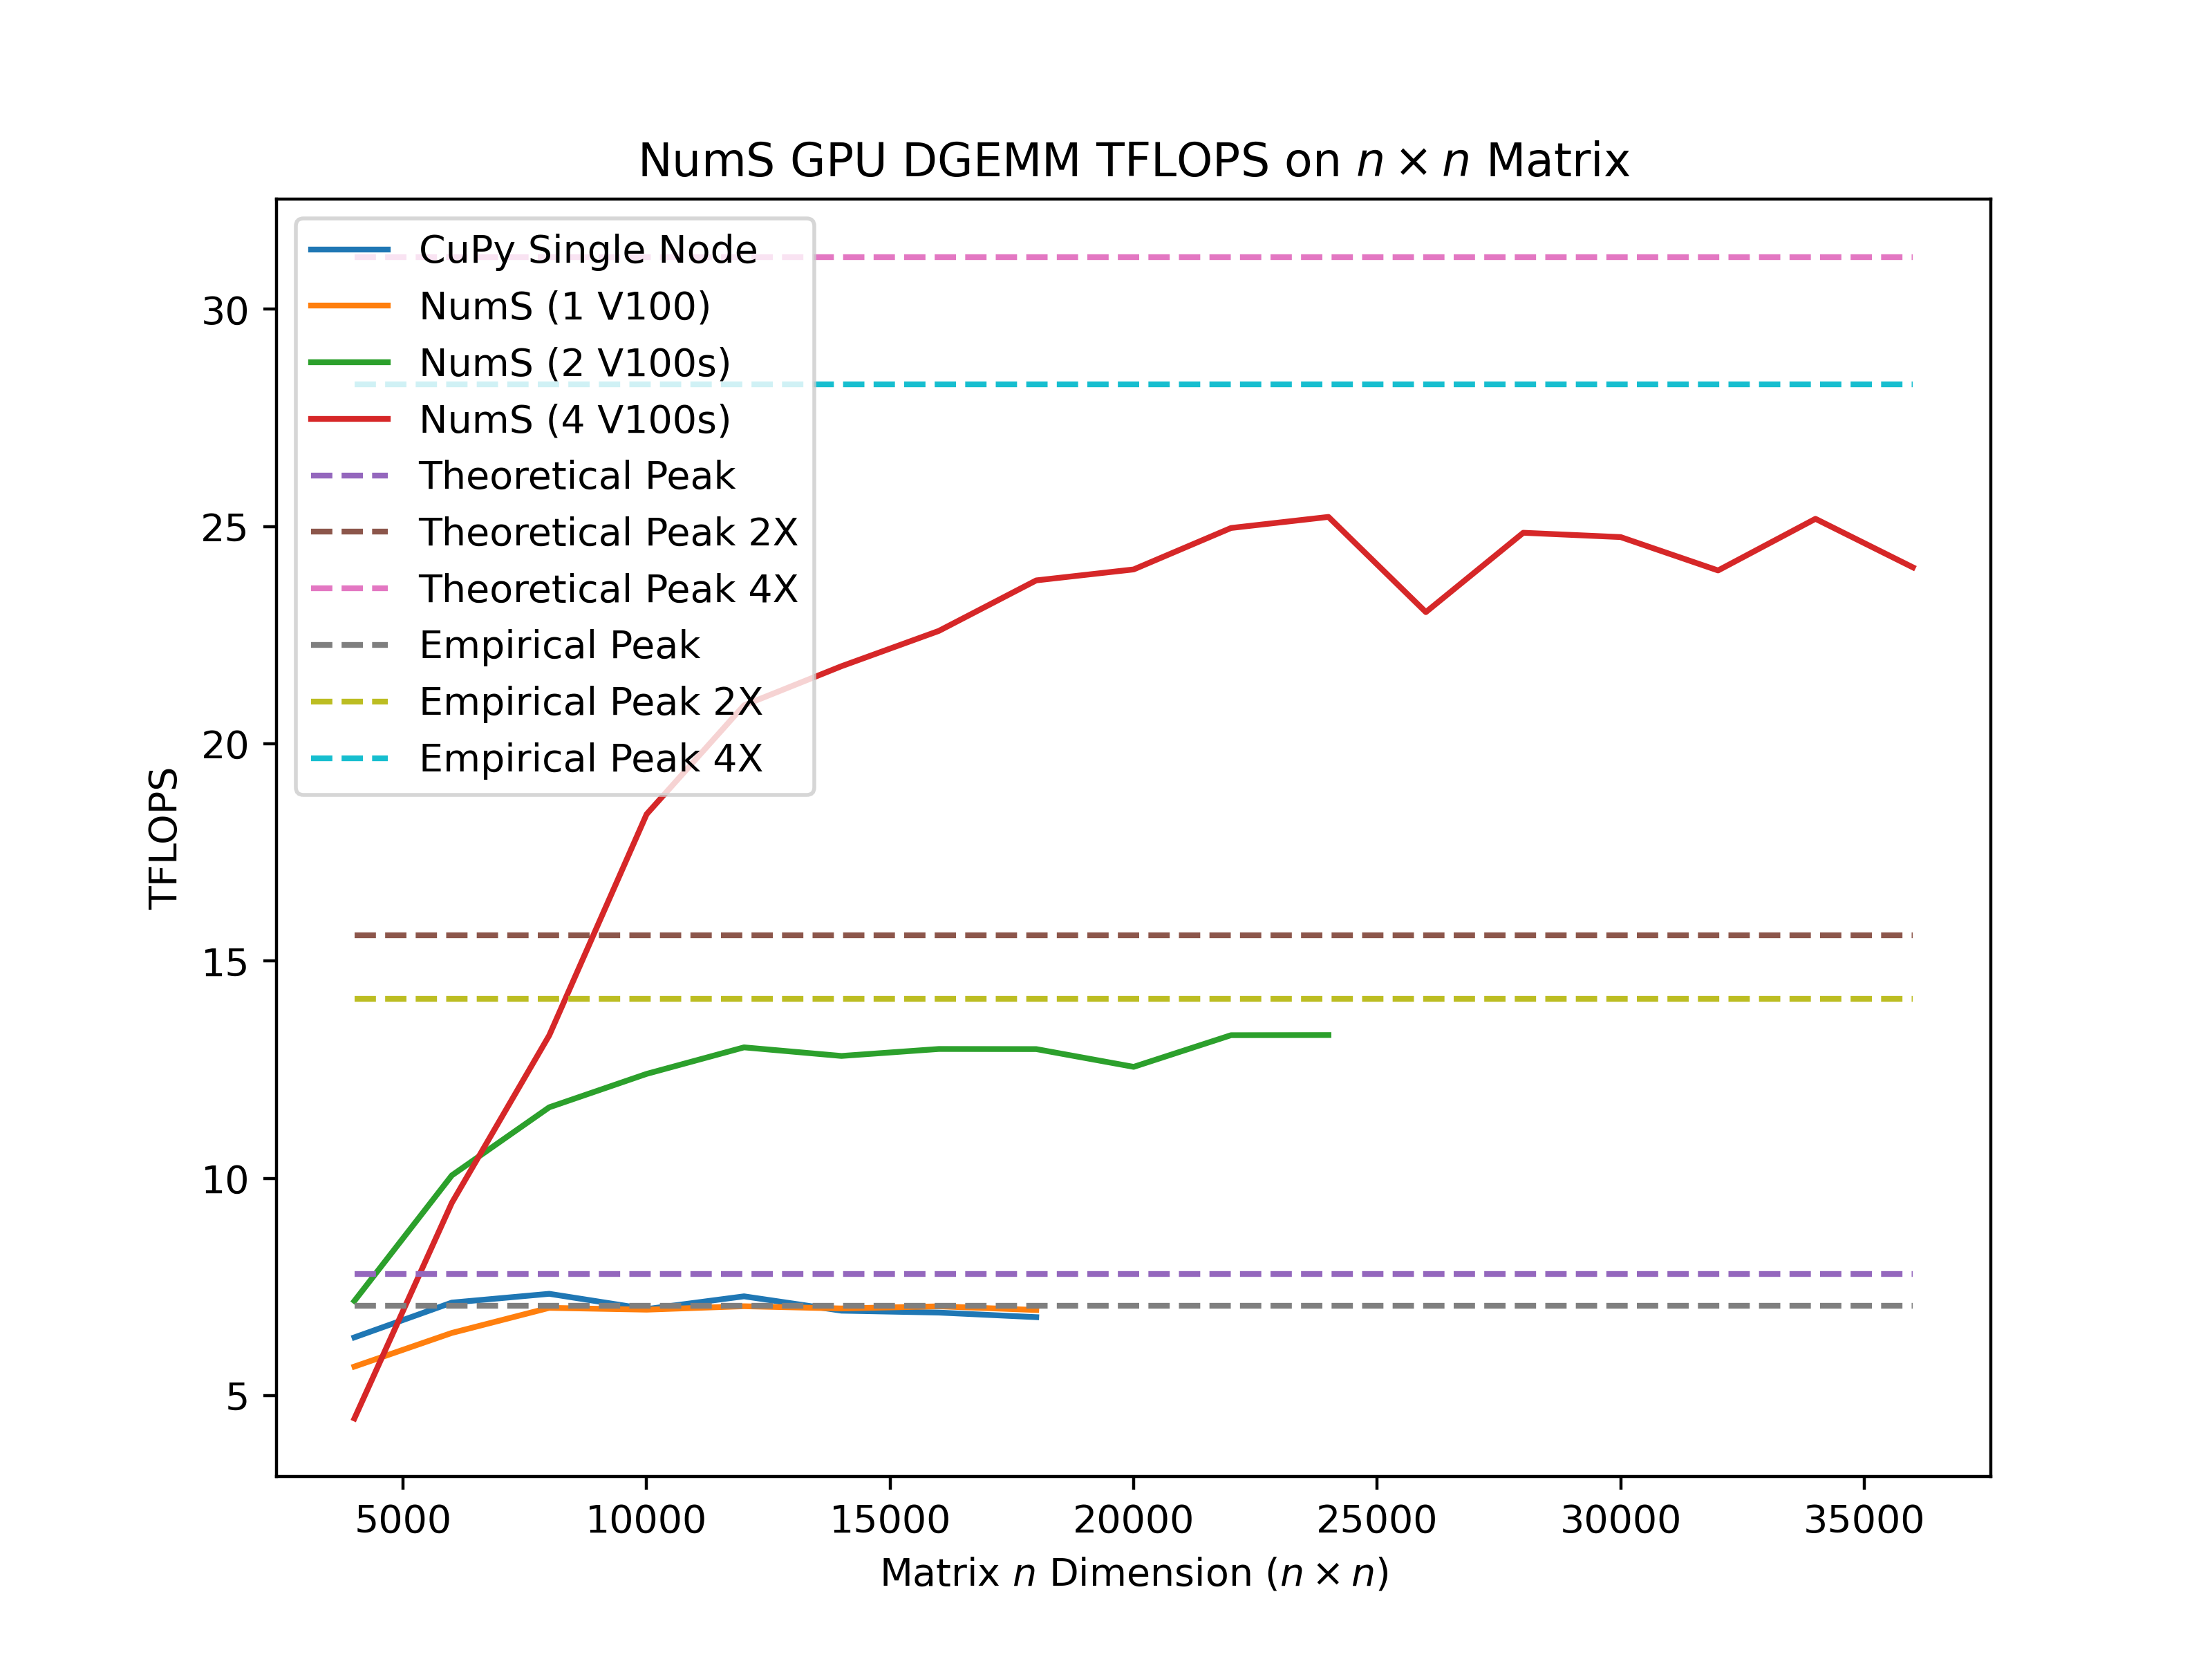
\includegraphics[width=5in]{figures/NumS_GPU_TFLOPS_DGEMM.png}}
  \caption{TeraFLOPs DGEMM Benchmark (Missing data in graph is OOM)}
  \label{fig:dgemm}
\end{figure}

\subsection{SGEMM}
The theoretical peak of NVIDIA V100 for single precision floating point numbers become nearly twice, 15.7 TFLOP/s. The same sizes are tested as NumS by default generates random double precision floating point numbers. We only transform matrices $A, B$ to single precision after they have been generated. Figure \ref{fig:sgemm} shows SGEMM performance on NumS up to 4 GPUs. NumS peak performance maintains 80.84-90.18\% of the theoretical peak in single precision performance. This is very similar performance from the DGEMM, and we see that the difference in precision scales well.

\begin{figure}
  \centerline{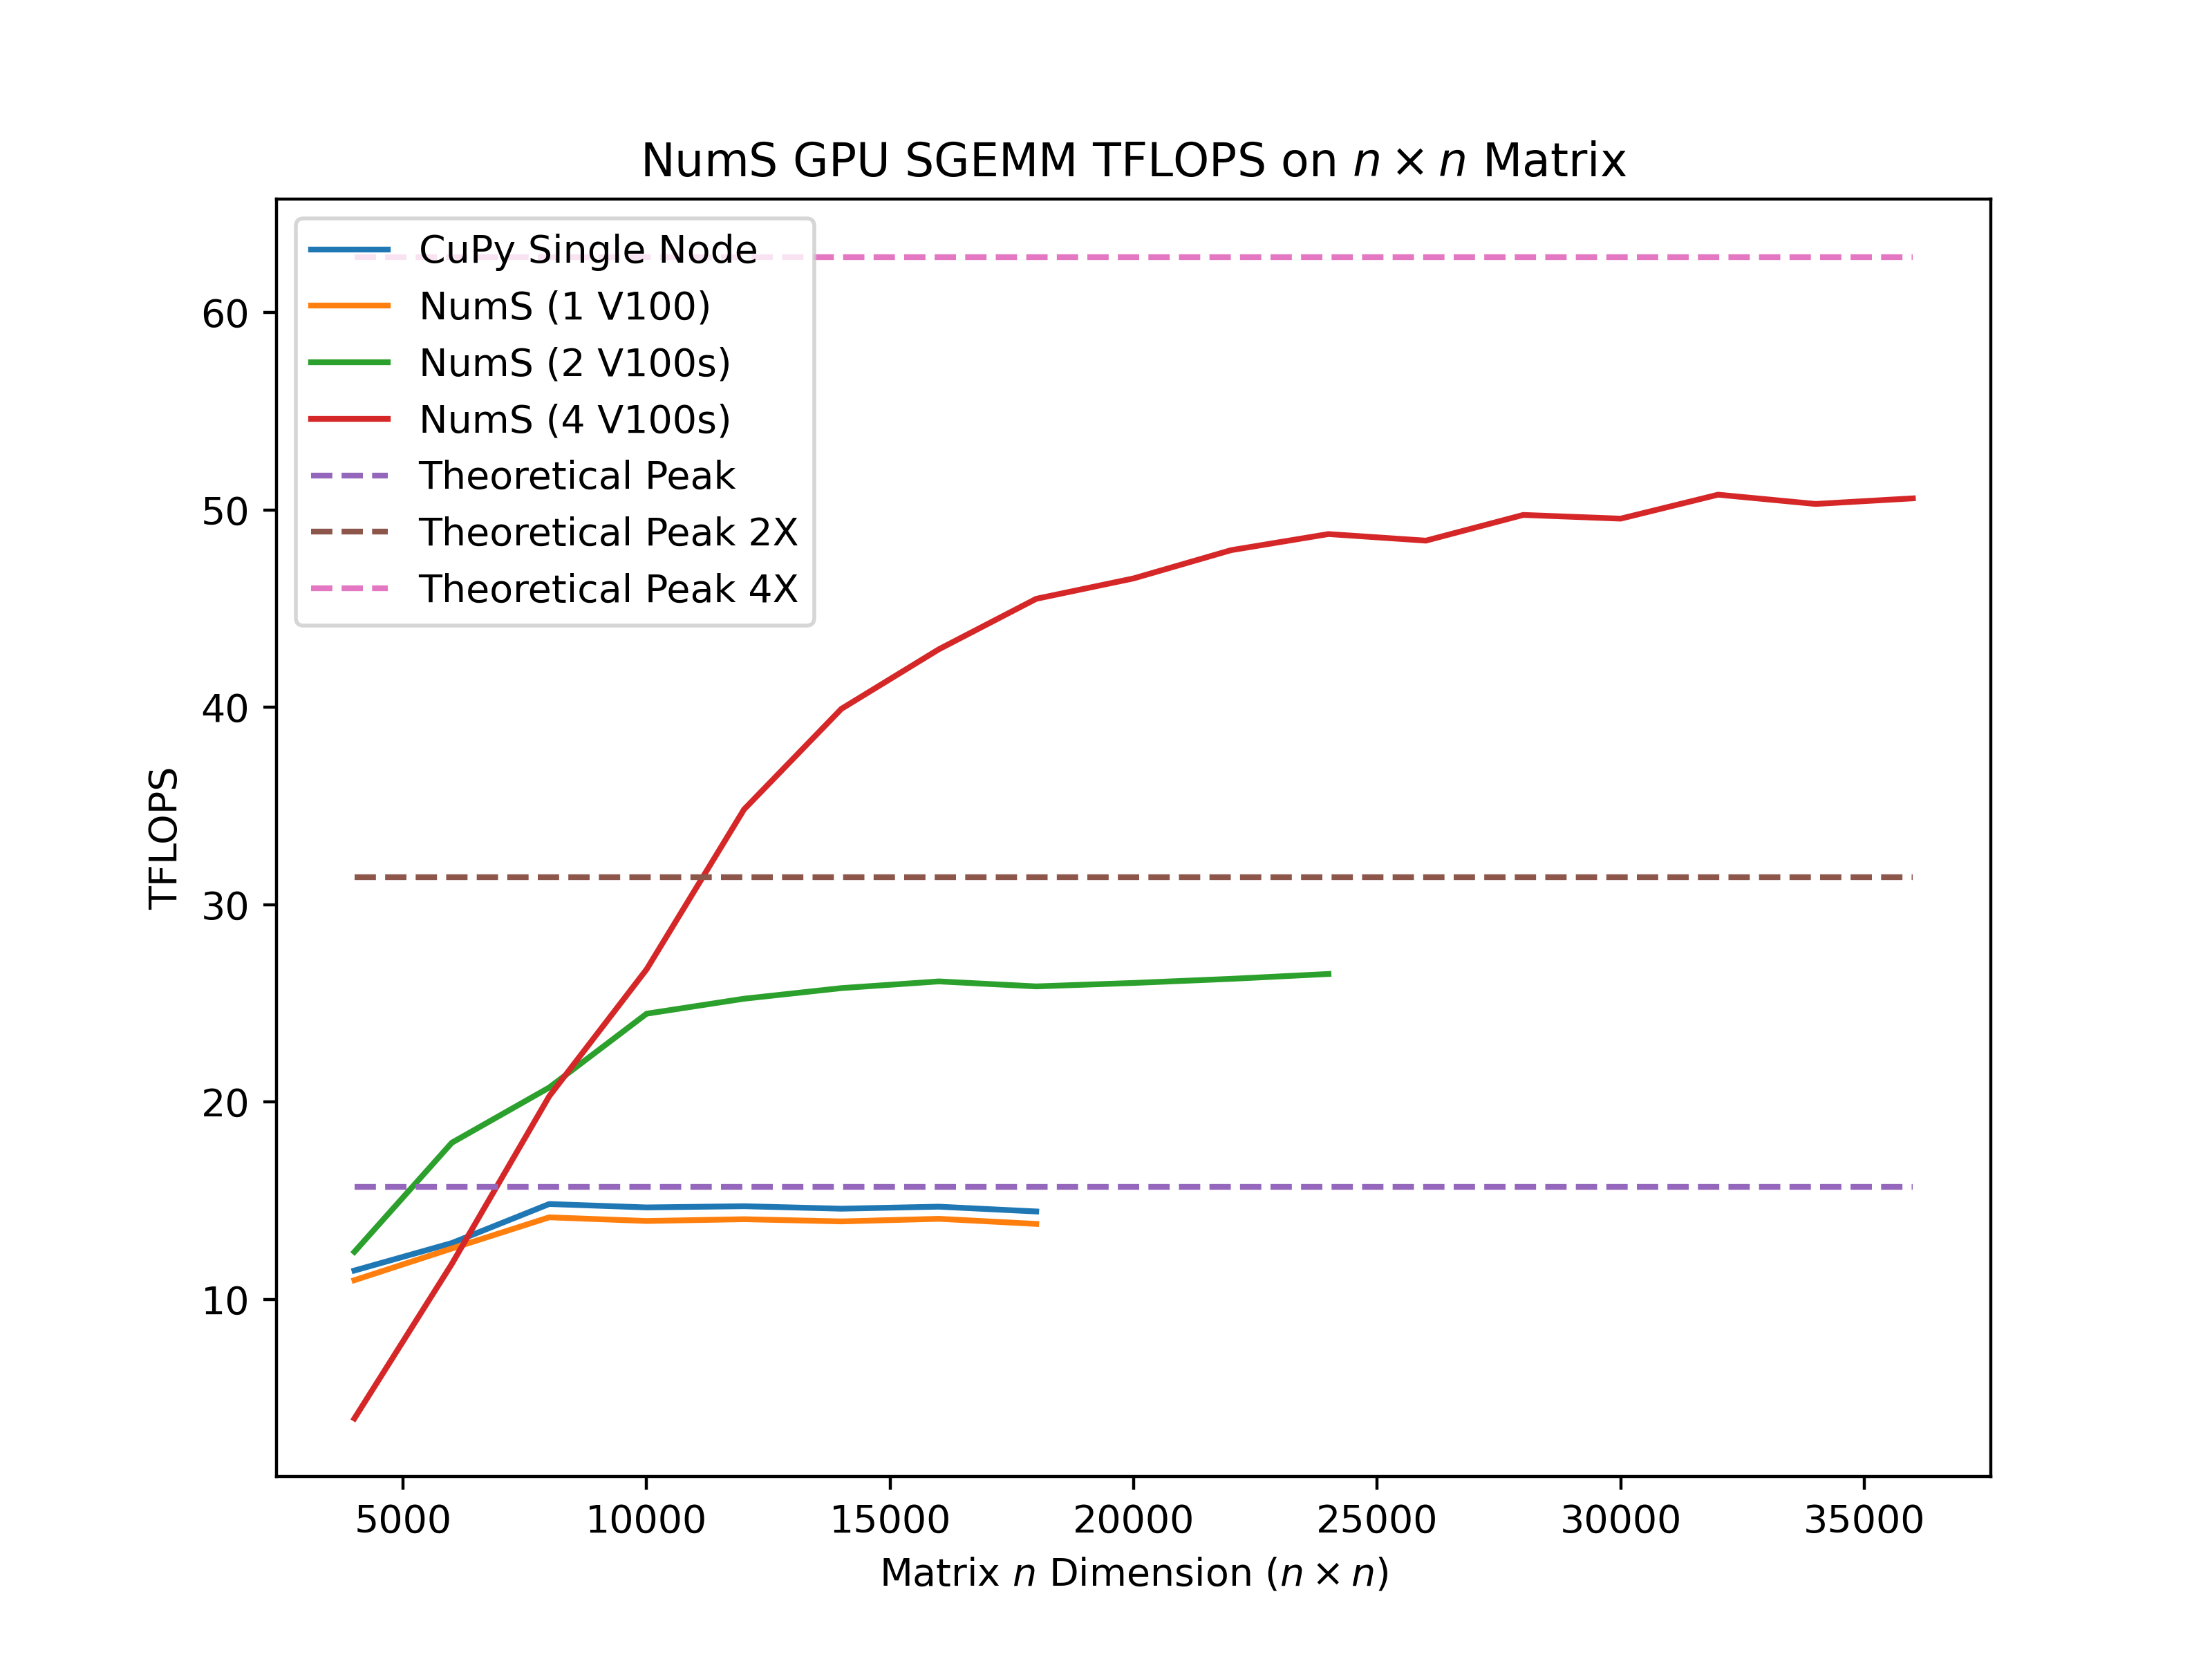
\includegraphics[width=5in]{figures/NumS_GPU_TFLOPS_SGEMM.png}}
  \caption{TeraFLOPs SGEMM Benchmark}
  \label{fig:sgemm}
\end{figure}

\subsection{Half Precision FP16 GEMM}
Half precision computations are useful where high precision doesn't matter and speed is important. NVIDIA V100 architecture is able to provide Tensor Cores 

Figure \ref{fig:fp16gemm} shows the performance

NumS peak performance maintains between 54.78-77.44\% of the theoretical peak for Tensor Cores. Unfortunately, when scaling to more than 1 GPU, the efficiency goes down. There is still more work to be done here to understand why scaling is not as efficient.

CPU architectures and software are not well supported for these types of computations. For example, NumPy cannot compute FP16 as many Intel architectures do not support \verb|fmadd| for 16 bit vectors. 


\begin{figure}
  \centerline{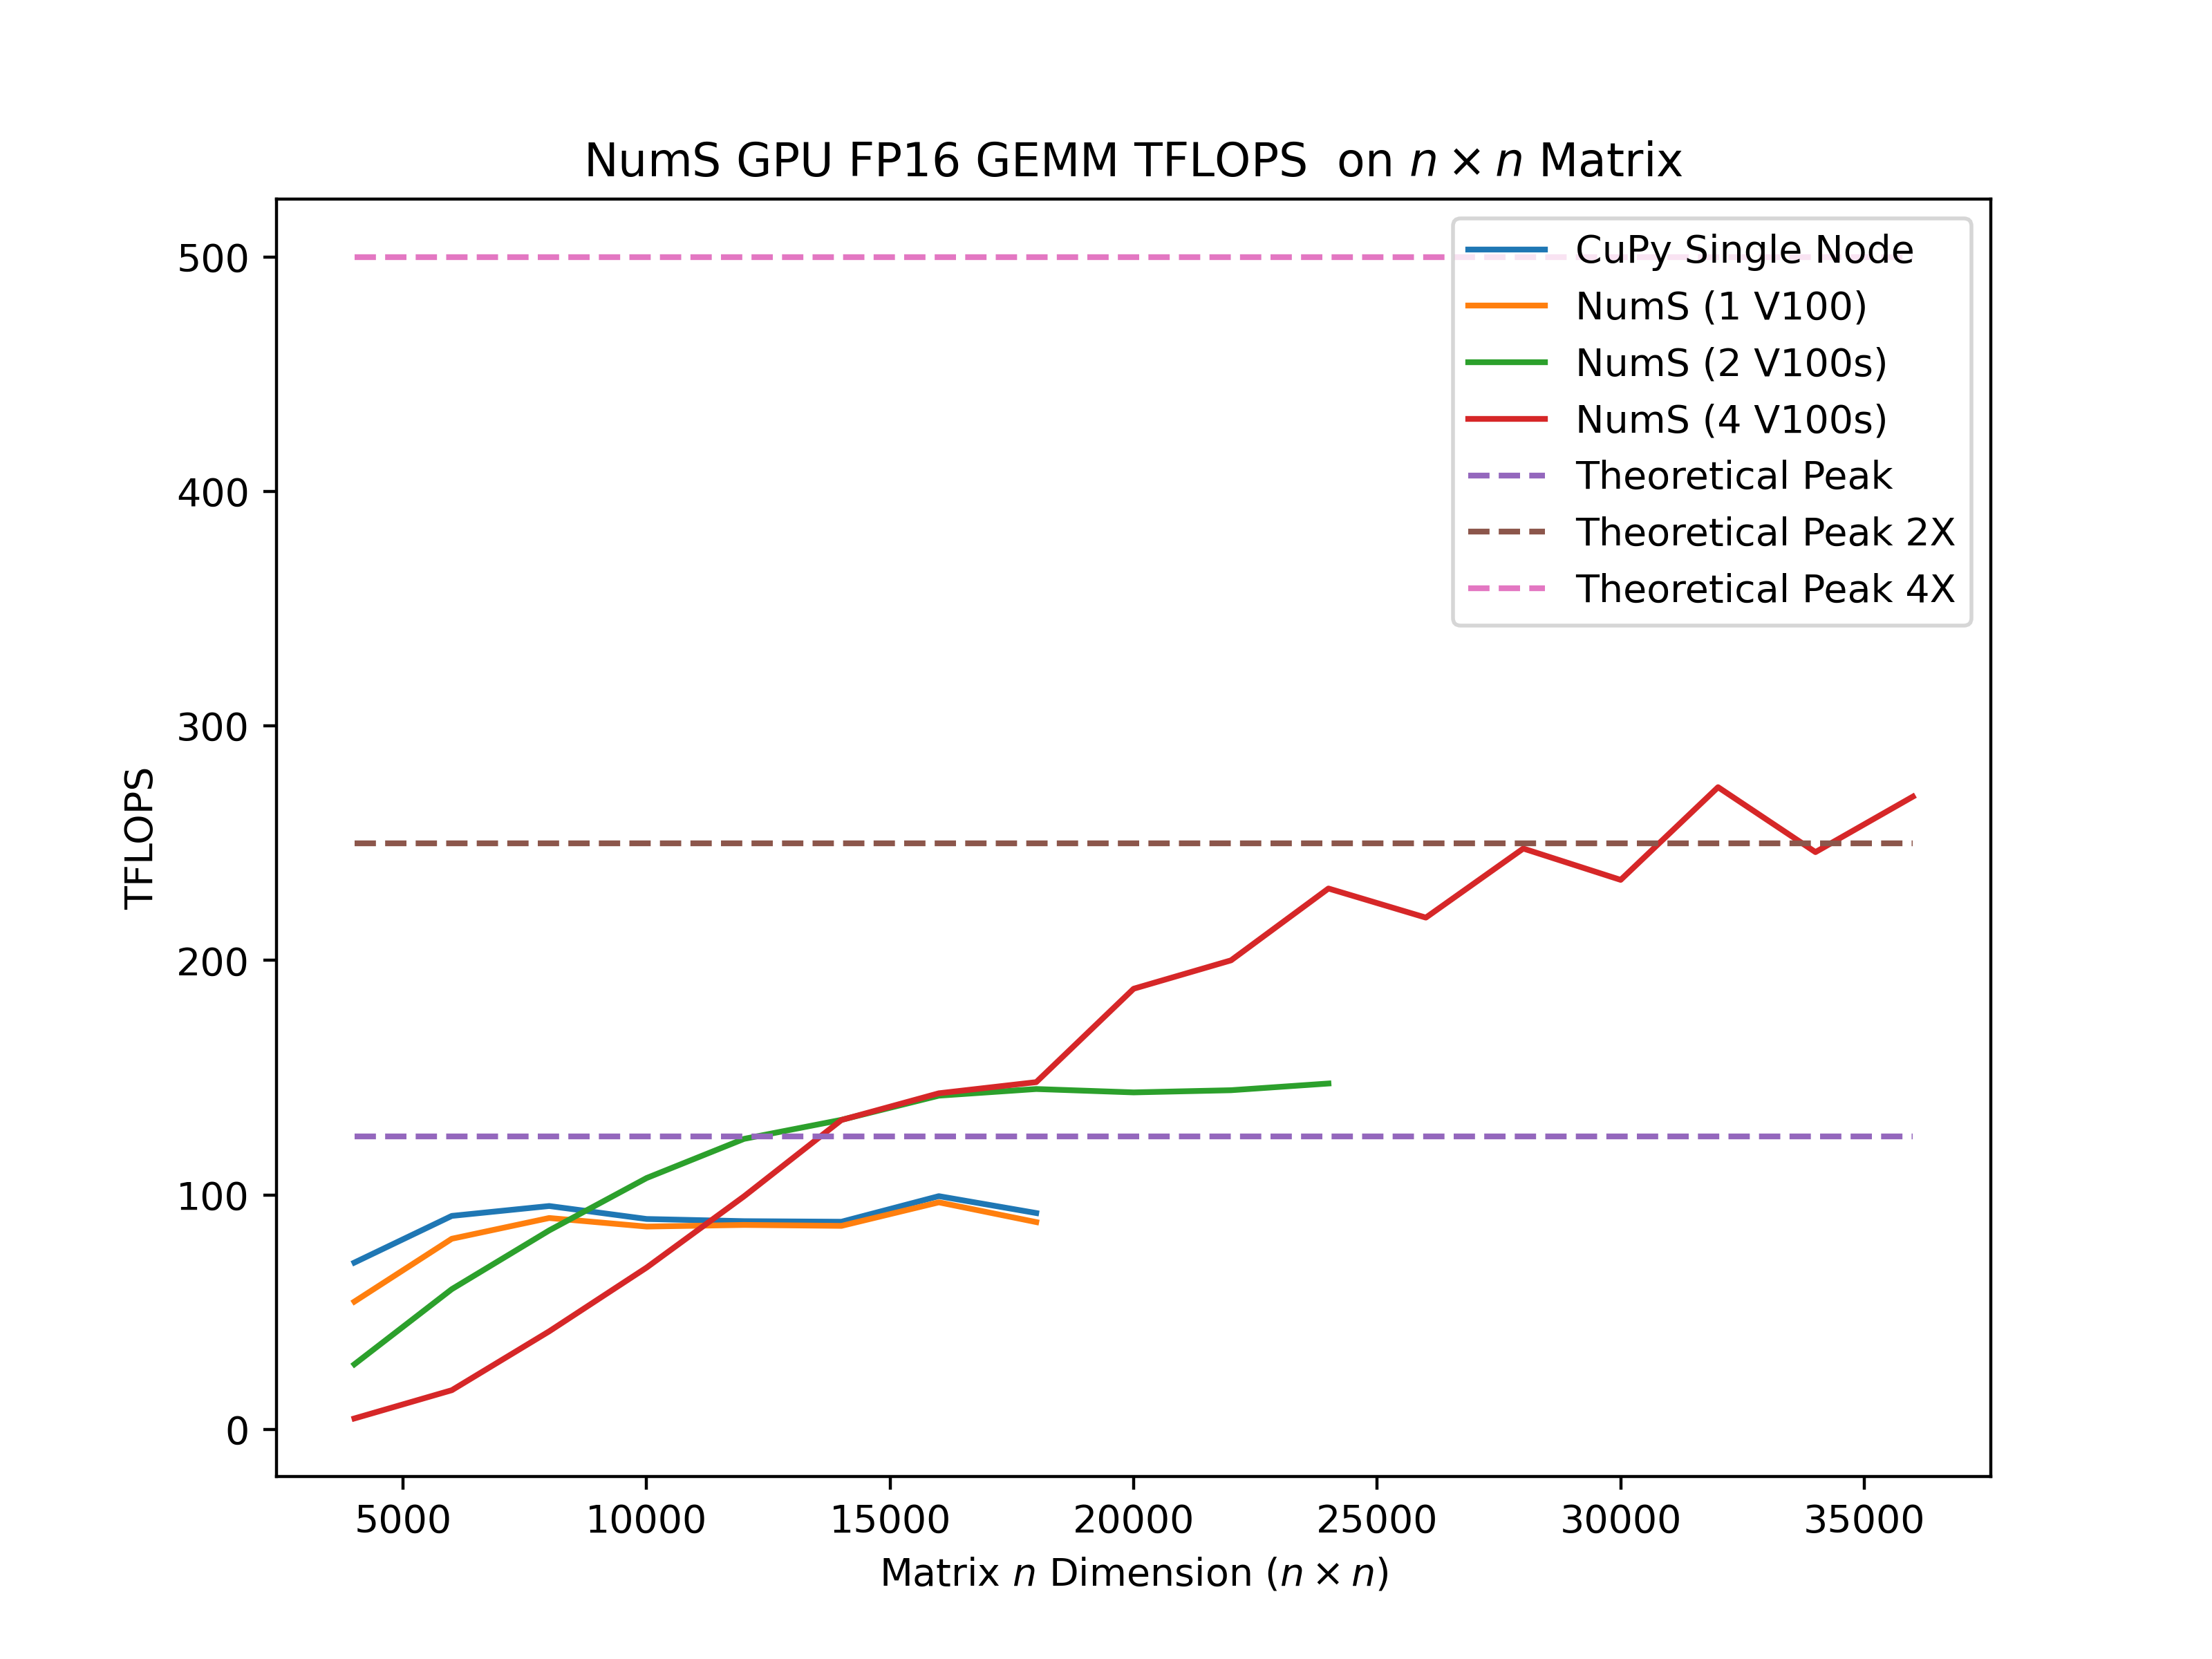
\includegraphics[width=5in]{figures/NumS_GPU_TFLOPS_FP16GEMM.png}}
  \caption{TeraFLOPs Half Precision (FP16) GEMM Benchmark}
  \label{fig:fp16gemm}
\end{figure}


\subsection{Elementwise Operations}
here we show that the 
Note that elementwise operations are handled by just CuPy and its internal CUDA API calls-- cuBLAS is not being used. Although the elementwise does not quite reach the theoretical peak, compared to just the normal CuPy implementation, it scales fairly well. 
 
%TODO weak scaling plots

\subsection{Logistic Regression}

\subsection{Multi Layer Perceptron}


\section{Related Work}
For executing linear algebra in a multi-GPU systems, we see that it is still novel and in it's early stages. For example, NVIDIA's cuBLAS Multi-GPU Extension is still in it's Early Access phase to limited group of developers. \cite{cublasmg} Dask also provides multi GPU support.

https://docs.rapids.ai/api/dask-cuda/nightly/index.html

\section{Conclusions}
Although we are able to achieve good scaling with non communication algorithms, we find the performance on communication algorithms a challenge, such as matrix multiply. The limitation is not as easy to pinpoint as it could come from NVIDIA's NCCL library performance or the design of NumS. 

Adding GPU support also allows users to run hardware agnostic code when using NumS. For example, a user can train on cheap distributed instances using CPU and Ray backend, and for inference, where performance is often crucial, they can switch to a GPU backend. 

\section{Future Work}
We wish to explore how to extend scalability to even more GPUs and to inter-node systems. The main challenge in properly designing such a system is efficiently scheduling within intra-node and between inter-node. We also only focused on HPC systems with the use of Bridges-2. But other work could be done to also try to deploy this on AWS cloud services, as they also provide V100 instances with P3 instances. 


the main challenge in impelmenting this backend so far has been trying to optimize communication bandwidths using nvlink connenctions and non blocking communicaiton. 
https://docs.rapids.ai/api/dask-cuda/nightly/index.html

\bibliographystyle{ieeetr}
\bibliography{references} 

\end{document}
